\chapter{Results of experiments with \grp}
\label{app:grp}
\textit{In this appendix results values of experiments with \grp{} are presented.}
\vfill
\newpage

Column labels:
\begin{itemize}
\item \texttt{Using Tabu List (no communication)}: Experiment in parallel using a global tabu list.
\item \texttt{Without Tabu List (no communication)}: Experiment in parallel without using a global tabu list.
\item \texttt{Using Tabu List (communication 1-1)}: Experiment in parallel using a global tabu list and communication \textit{one~to~one}.
\item \texttt{Using Tabu List (communication 1-n)}: Experiment in parallel using a global tabu list and communication \textit{one~to~N}.
\item \texttt{Sequential (without tabu list)}: Experiment using one core and without tabu list.
\item \texttt{Sequential (with tabu list)}: Experiment using one core and a global tabu list.
\item \texttt{time}: Time in milliseconds. 
\item \texttt{iterations}: Number of iterations.
\item \texttt{restarts}: Number of restarts performed by the winner solver.
\end{itemize}

Color caption:
\begin{itemize}
\item \gracias{Values in red color}: A receiver solver was the winner, finding the solution thanks to the received information.
\item \sender{Values in blue color}: A sender solver was the winner.
\item \nocomm{Values in black color}: A non-communicating solver was the winner.
\end{itemize}

Other captions:
\begin{itemize}
\item \texttt{Eps}: The gap ($\epsilon$) used to consider a configuration near enough to a possible local minimum.
\item \texttt{Norm}: The vector norm type used to compute the mentioned gap.
\item \nocomm{tabu size}: The capacity of the global tabu list.
\end{itemize}

%\noindent\rule[2pt]{\textwidth}{0.8pt}

\clearpage
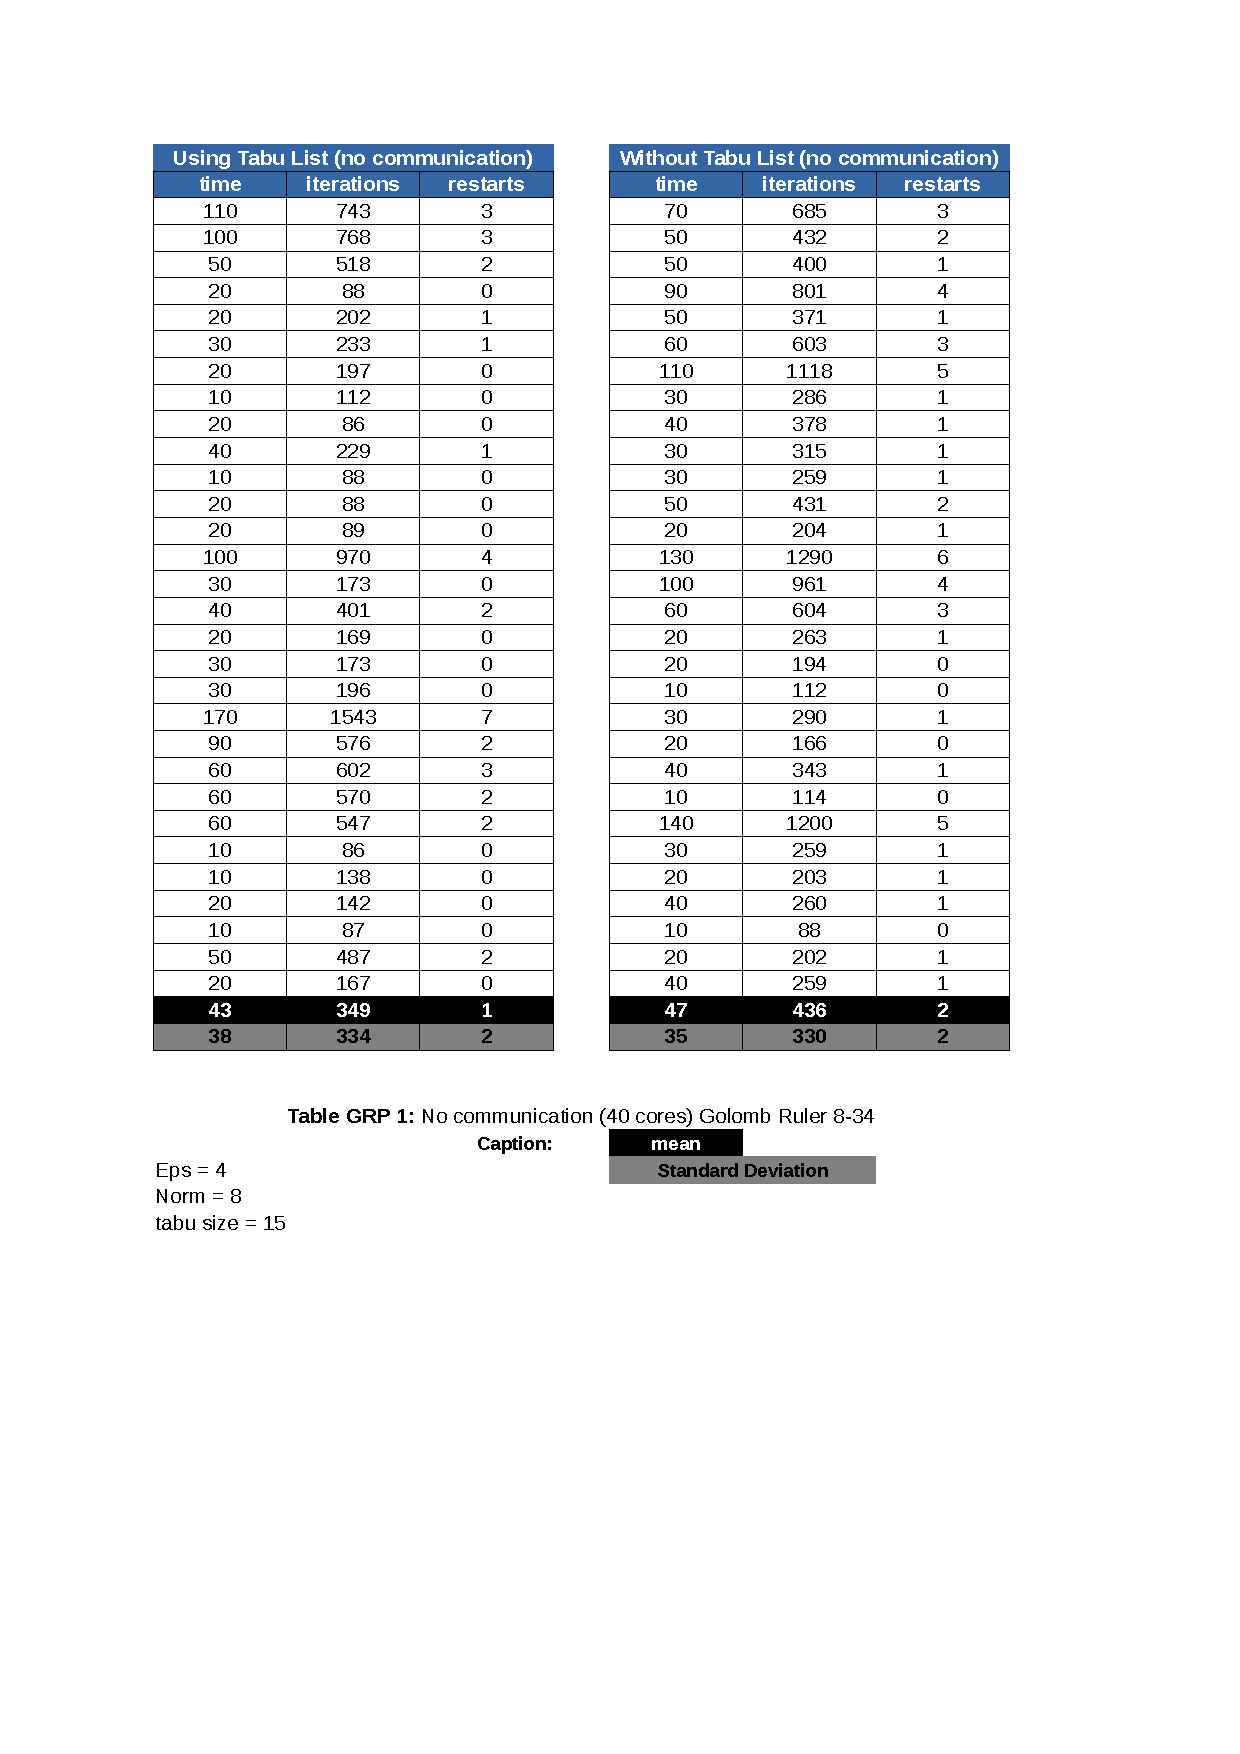
\includepdf[pages=-]{appres//res_golomb.pdf}